\section{Who had the most positive influence on you as a child?}
I'm choosing to write about a group of people who had an influence on me as a child.
This is a group of people that I did not choose to know, they were given to me.
This group is the five brothers and five sisters who grew up with me.
Seven were older than me and three younger than me.
My oldest brother is ten years older than me and my youngest sister is seven years younger than me.
It was this group of people who set the tone for the environment in which I lived for the first twenty-four years of my life.
Work was a part of this influence.
My older siblings supervised the younger siblings when working.
My older brother Dave even took it upon himself to discipline us when he felt we were not doing the job to his expectations.
A rubber hose was used.
When it was time for me to get a job away from home I followed my older siblings by taking the jobs they had moved on from.

But the question asked for "the most positive influence" so here are some memories for that.
They set a positive expectation regarding school and friendship.
Good grades were expected and most of them demonstrated that good grades could be achieved.
Making friends was important and my older sister Martha made friendship look like so much fun.
During her high school years she became part of a group of 13 friends who had good times and adventures together.
Hearing about the overnight slumber parties they had left me longing for a group of friends like she had.
\begin{figure}
\centering
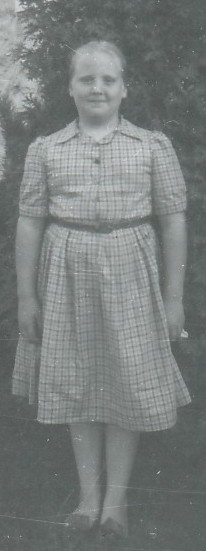
\includegraphics[width=0.9\textwidth]{childhood/20.jpg}
\caption{
Taken after Mom's funeral 2008.
}
\end{figure}

My siblings demonstrated what it meant to think for themselves by not following exactly in the path our parents expected.
When they started dated they provided an education in how that was done and chose partners who became a significant part of the family.
When they had children they provided an example of how to parent.
They provided examples of how to live as responsible adults.
They each have enriched my life tremendously and left a significant imprint on my life.
I'm grateful to have grown up in this large family.
\begin{figure}
\centering
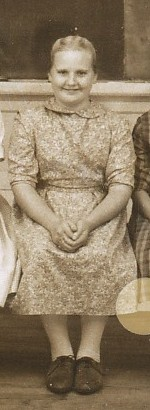
\includegraphics[width=0.9\textwidth]{childhood/21.jpg}
\caption{
The siblings taken at NDMS January 2010.
}
\end{figure}

\textbf{From Abby -} Thanks for this lovely response Mom.
It makes a lot of sense that your older siblings played such a big role in your life by providing examples of future stages of life.
I would be curious about what your experience was like with some of your younger siblings.
Do you feel like they influenced you in terms of how you learned to nurture or instruct others? Obviously most of your siblings were older than you, but I would be curious to learn more about how you related to Joe, Rachel and Esther.

\textbf{From Mom -} Interesting question Abby.
My relationship with my younger siblings is different than that with my older siblings.
I find that I feel protective of my younger siblings.
I also realize that I do not remember details of what happened in their lives once I hit the high school years and was preoccupied and distracted with my own life.
As with all of my siblings there was a time of realizing what it meant to be adults together.
I enjoy the ongoing opportunity of trying to stay connected and up to date with what is happening in their lives.
Family does not go away and is a great resource of relationships.
Rachel had become one of my favorite sisters to talk with.
Joe and I now share a diagnosis.
I admire Esther's determination to live her life with meaning.
Each of them influences me in their unique way.
They each have a distinct sense of humor which I enjoy and admire.
While Rachel and I share a lot of interests and concerns, Joe and Esther likely have more differences of perspective.

